\chapter{Linked Connections}
\label{lc}

Linked Connections \cite{colpaert_iswc_2015} is een framework die \textit{client-side} routeplanning mogelijk maakt. Volgende sectie verduidelijkt hoe de huidige implementatie werkt. Vervolgens wordt uitgelegd hoe connecties worden gegenereerd uit een GTFS feed. Ten slotte wordt verduidelijkt hoe intermodaal routeplannen werkt.

\section{Principe}

Stel je voor dat je de tram moet nemen naar je werk: je stapt ergens op, wacht vijf stophaltes en aan de zesde stophalte stap je af. Dit is een route die uit zes connecties bestaat. Een connectie is de verbinding tussen een vertrek- en eindstop zonder onderbreking. Bij zo'n connectie horen respectievelijk ook een vertrek- en aankomsttijd. Een route kan berekend worden met het CSA algoritme (zie \ref{csa}) die een query en een gesorteerde lijst op vertrektijd als inputwaarde vereist.

Een Linked Connections server presenteert deze gesorteerde connecties in de vorm van Linked Data Fragments (\ref{ldf}) aan de cli\"ent. Momenteel is het enkel mogelijk om de vertrektijd van een query mee te geven als parameter. Met behulp van texttit{hydra:nextPage} links kan de cli\"ent makkelijk opeenvolgende fragmenten ophalen. (zie figuur \ref{lcfragmenten}).

\begin{figure}[h!]
\centering
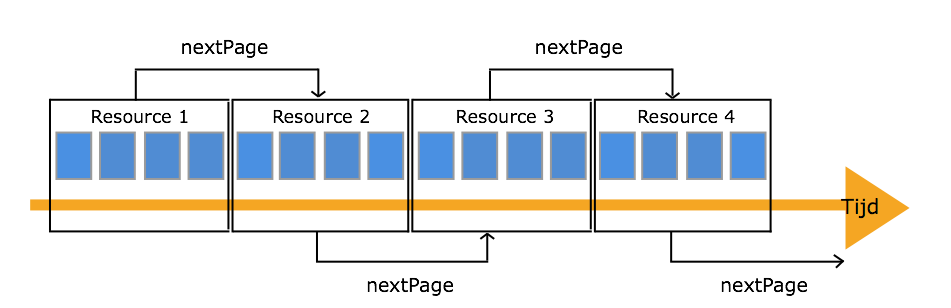
\includegraphics[width=0.8\textwidth]{hypermediafragmenten.png}
\caption{Connecties zijn gesorteerd onderverdeeld in fragmenten die verbonden zijn met hydra:nextPage links.}
\label{lcfragm}
\end{figure}

\begin{lstlisting}[label=queryconnecties,caption=HTTP URL van fragment met Linked Connections.]
http://voorbeeld.org/connecties?vertrekTijd=2015-10-21T11\%3A30
\end{lstlisting}

Het publiceren van de data gebeurt met behulp van drie technologi\"een: 
\begin{itemize}
\item REST zorgt ervoor dat resources cachebaar zijn. Hier zijn fragmenten de resources. Het aantal mogelijke URI's is afhankelijk van het tijdsinterval van de fragmenten. Als T het tijdsinterval in minuten is van de fragmenten, dan kan het aantal mogelijke URI's berekend worden met formule \ref{lc:aantalurisoorspronkelijk}.
\begin{equation} \label{lc:aantalurisoorspronkelijk}
24 * 60 / T
\end{equation}

Als T = 10 min, dan zijn er 144 verschillende fragmenten. De meeste ov-bedrijven rijden niet 24/24 dus in praktijk zijn er nog minder fragmenten. Met behulp van HTTP omleidingen kan dit opgelost worden.
\item Hypermedia zorgt niet enkel voor het vinden van volgende fragmenten, maar ook voor het makkelijk uitbreiden van connecties. Dit kan gaan van een koppeling met geonames tot koffiebars in de buurt.
\item Het semantisch web zorgt voor de semantische interoperabiliteit van de connecties en de API. Dit laat toe om generische clients te bouwen.
\end{itemize}

Op de LDF-as (zie \ref{ldf-lc5}) staat huidige implementatie aan de linkerkant. Het kost de server weinig moeite om data te publiceren door de hoge cachebaarheid. Een cli\"ent moet daarentegen veel connecties scannen om tot een route te komen. Later (\ref{resultaat-origineel}) zal de exacte performantie verduidelijkt worden.

\begin{figure}[h!]
\centering
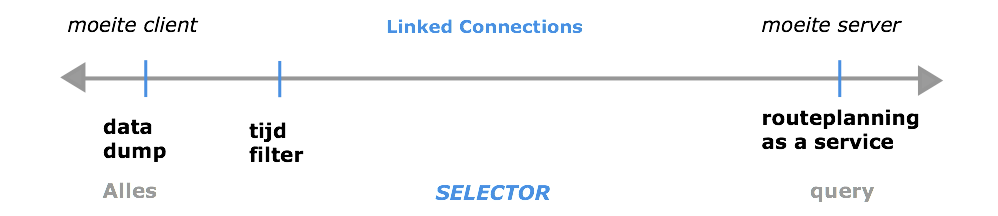
\includegraphics[width=0.8\textwidth]{LDF-as5.png}
\caption{Linked Data Fragmenten-as met Linked Connections}
\label{ldf-lc5}
\end{figure}

\section{Voorbewerking}

Gelinkte connecties worden berekend uit een GTFS \textit{feed}. De convertor in deze masterproef maakt gebruik van een MySQL-databank om queries op uit te voeren. \footnote{Ondertussen is een veel snellere convertor gemaakt die volgens een ander principe werkt, zonder databank. Zie github.com/linkedconnections/gtfs2lc} Het is belangrijk op te merken dat connecties niet gesorteerd moeten zijn bij het voorbewerken. Deze worden later in de databank van de Linked Connections server ingeladen die zelf sorteert. Figuur \ref{inladengtfs} toont een overzicht van de verschillende stappen om connecties te genereren.

\begin{figure}[h!]
\centering
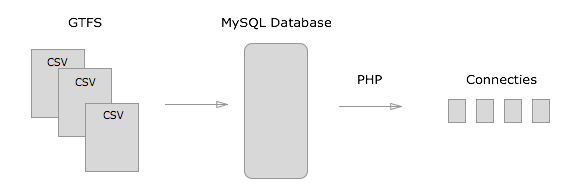
\includegraphics[width=1.0\textwidth]{Preprocessor.png}
\caption{Overzicht hoe connecties worden gegenereerd uit een GTFS feed. Deze wordt ingeladen in een MySQL databank. Met de scripttaal PHP worden connecties gegenereerd hieruit.}
\label{inladengtfs}
\end{figure}

Connecties worden dag per dag berekend. Ofwel worden start- en einddatum meegegeven als parameters, ofwel worden start- en einddatum van de GTFS feed zelf genomen. Vervolgens worden alle services uit \textit{calendar} en \textit{calendar\_dates} van een bepaalde dag opgehaald. Bij elke service hoort een bepaalde \textit{route} en een verzameling \textit{trips} die dan worden opgehaald uit \textit{trips}.
Een laatste stap is het overlopen van \textit{stoptimes.txt}. Uit de combinatie van twee opeenvolgende stoptimes kan een connectie berekend worden. Lijst \ref{vbstoptimes} bevat een voorbeeld van twee opeenvolgende stoptijden van een bepaalde trip.

\begin{lstlisting}[label=vbstoptimes,caption=Vereenvoudigde stoptimes in CSV.]
trip_id,arrival_time,departure_time,stop_id,stop_sequence
16,07:18:00,07:18:00,8200100,1
16,07:33:00,07:33:00,8200110,2
\end{lstlisting}

\begin{figure}[h!]
\centering
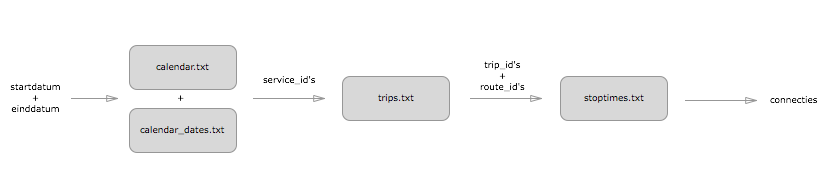
\includegraphics[width=0.8\textwidth]{volgordeconvertor.png}
\caption{Per dag worden de corresponderende service ID's, trip ID's en route ID's berekend. De vertrek-/aankomststopplaats met respectievelijk vertrek-/aankomsttijd worden berekend uit een verzameling stoptimes. }
\end{figure}

Codevoorbeeld \ref{connectiejsonld} toont hoe een connectie eruit ziet bij output. Merk op dat een '@context' niet is toegevoegd en ook niet in een graaf zit. In subsectie \ref{jsonldstream} wordt hierover meer uitleg gegeven.

\begin{lstlisting}[label=connectiejsonld,caption=Connectie voor een bepaalde trip met bijkomstige route in JSON-LD.]
{	
	"@id": "http://example.org/connections/1"
	"@type": "http://semweb.mmlab.be/ns/linkedconnections#Connection",
	"http://vocab.gtfs.org/terms#trip": "16",
	"http://vocab.gtfs.org/terms#route": "route-1",
	"http://semweb.mmlab.be/ns/linkedconnections#departureTime": "2015-10-21T06:18:00.000Z",
	"http://semweb.mmlab.be/ns/linkedconnections#departureStop": "8200100",
	"http://semweb.mmlab.be/ns/linkedconnections#arrivalTime": "2015-10-21T06:33:00.000Z",
	"http://semweb.mmlab.be/ns/linkedconnections#arrivalStop": "8200110"
}
\end{lstlisting}

De tijdszone van vertrek- een aankomsttijd staat in Coordinated Universal Time (UTC). Er moet altijd rekening gehouden worden met de tijdszone van de GTFS feed. In dit voorbeeld \ref{vbstoptimes} werd een feed uit Belgi\"e genomen. Om de Belgische tijd (UTC+1) om te zetten naar UTC moet er een uur afgetrokken worden van de tijd die vermeld staat in GTFS stoptijden.

Een van de moeilijkheden voor het genereren van connecties was het ophalen van trips die voor middernacht vertrekken, en dus geclassificeerd zijn onder die dag, maar na middernacht pas stoppen. GTFS lost dit op door de tijd na middernacht door te tellen, bijvoorbeeld 2u 's nachts staat weergegeven als 26u. Volgens GTFS rijden deze stoptimes allemaal op dezelfde dag, maar voor Linked Connections zijn dit effectief twee verschillende dagen, omdat er met exacte tijden gewerkt wordt.
Om dit op te lossen worden er twee extra vlaggen toegevoegd in de databank of de vertrek- en aankomsttijd van een stoptijd voor of na middernacht plaatsvinden.

Een databank gebruiken heeft als grote nadeel dat de data ingeladen moet worden vooraleer berekeningen kunnen plaatsvinden. In \ref{table:inladengtfs} staat een overzicht van de drie gebruikte datasets in deze masterproef met de tijd om in te laden. Voor zeer grote datasets, zoals De Lijn, is inladen een bottleneck.

\begin{table}[htbp]
\centering
\begin{tabular}{ | l || c | c | c |}
  \hline			
    & Tijd (min) & Grootte (MB) & Periode (weken) \\ \hline
  NMBS & 3.1 & 1.1 & 12  \\
  NS & 8.35 & 21.4 & 56 \\
  De Lijn & 100 & 44 & 10 \\
  \hline  
\end{tabular}
\caption{Tijd om een GTFS feed in te laden in een MySQL databank.}
\label{table:inladengtfs}
\end{table}

Het genereren van connecties zelf gaat een stuk rapper. In \ref{table:connectiesgenereren} zie je dat voor kleine datasets (zoals NMBS en NS) het minder dan minuut duurt om de connecties voor een dag te berekenen. De Lijn scoort opnieuw zeer slecht door de grootte van de dataset.

\begin{table}[htbp]
\centering
\begin{tabular}{ | l || c | c | c |}
  \hline			
    & Tijd (min) & Connecties \\ \hline
  NMBS & 0.21 & 55479 \\
  NS &  &  \\
  De Lijn & 14.97 & 1049186 \\
  \hline  
\end{tabular}
\caption{Tijd om connecties te genereren voor een dag.}
\label{table:connectiesgenereren}
\end{table}

\subsection {JSON-LD stream}
\label{jsonldstream}
Om de connecties als Linked Data te publiceren werd er voor gekozen om JSON-LD te gebruiken. JSON wordt beschouwt als het \textit{de facto} standaardformaat op het web dankzij de compactheid, leesbaarheid en vele handige tools die hiervan gebruik maken. Wanneer een verzameling objecten dezelfde context heeft, zijn er twee mogelijkheden om deze te publiceren:
\begin{itemize}
\item een gemeenschappelijke context voorzien en alle objecten in bijhorende graaf steken (zie \ref{tripjsonldgraph}). Deze methode vereist dat de graaf in het geheugen geladen moet worden vooraleer verdere operaties mogelijk zijn.
\item elk object een context geven (zie \ref{tripjsonld}). Met deze methode kan object per object gestreamt worden, maar zorgt voor grote overhead door de context die telkens mee gepubliceerd wordt.
\end{itemize}
Een oplossing hiervoor is de JSON-LD streamspecificatie \footnote{https://github.com/pietercolpaert/jsonld-stream}. Deze geeft aan dat de context van een object met '@context' van toepassing is op alle andere objecten van het document. Zo moet er maar eenmalig een context opgegeven worden en wordt impliciet verondersteld dat de andere objecten deze context gebruiken.
De voorbewerker kan nu connecties als Linked Data wegschrijven zonder extra dataverlies en gestroomlijnd. Dit stroomlijnen is belangrijk om de data later lijn per lijn te kunnen inladen in een databank.

\section{Client}

De client is verantwoordelijk voor het berekenen van de snelste route. Deze kan met een paar lijntjes code aangemaakt worden (zie \ref{clientvb}).
\begin{lstlisting}[label=clientvb,caption=Code om client op te zetten in JavaScript.]
var planner = new window.lc.Client({"entrypoints" : ["http://example.linkedconnections.org/"]});
planner.query({
			"departureStop": "Brussel-Zuid",
			"arrivalStop": "Gent-Sint-Pieters",
			"departureTime": new Date("2015-11-05T10:00")
			}, function (stream) {
				stream.on('result', function (pad) {
					// pad bevat verzameling connecties die snelste route voorstellen
				});
			 	stream.on('data', function (connectie) {
			 		// connectie is gebruikt geweest voor minimale overspannende boom
			 	});
});
\end{lstlisting}
\label{vbclient}

Linked Connections van verschillende ov-bedrijven worden gedistribueerd opgesteld. De cli\"ent is verantwoordelijk voor het samenvoegen van connecties. In figuur \ref{overzichtclientserver} staat een overzicht van een client - meerdere servers opstelling. Rechts staan twee Linked Connection servers, de ene verantwoordelijk voor de connecties van een vervoersmaatschappij van bussen, de andere van treinen. Links staat een client die de fragmenten ophaalt van beide servers. Voor het scannen zelf kan plaatsvinden, moeten deze samengevoegd worden. Daarna kan de snelste route met Connection Scan Algorithm (CSA) gepland worden.

\begin{figure}[h!]
\centering
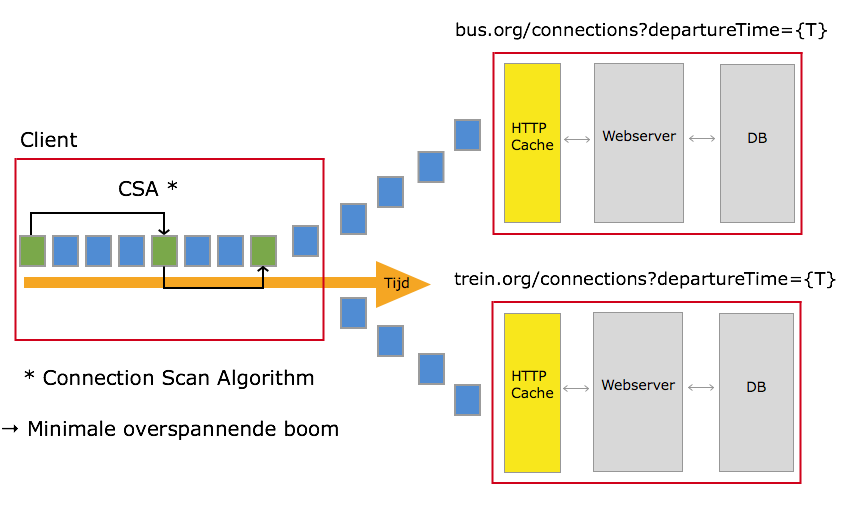
\includegraphics[width=0.5\textwidth]{OverzichtClientServer.png}
\label{overzichtclientserver}
\caption{Opstelling van een client en twee Linked Connections servers.}
\end{figure}

\subsection{Merger}

Een merger voegt meerdere stromen van gesorteerde connecties samen tot een stroom. Dit is noodzakelijk voor de cli\"ent om CSA te kunnen toepassen.

Connecties komen onder de vorm van een \textit{stream} binnen. Zo'n stream werkt asynchroon met events. Deze worden opgeworpen wanneer bijvoorbeeld data beschikbaar is. Figuur \ref{merger} toont een overzicht van een merger. Deze luistert (1) naar de verschillende datastromen tot deze data vrijgeven. De connecties worden toegevoegd in wachtrijen. Wachtrijen (2) hebben als voorwaarde dat ze zelf gesorteerd zijn. Datastromen worden telkens gepauzeerd na het opvangen van data. Dit is noodzakelijk om de cli\"ent beslissingstijd te geven. Zo kan er beslist worden om een bepaalde connectiestroom uit te schakelen of toe te voegen. Een andere reden waarom de merger de connectiestromen pauzeert, is het feit dat de wachtrijen minstens een connectie moet bevatten van elke connectiestroom. Wanneer de merger connecties teruggeeft, worden alle connecties van elke wachtrij met dezelfde lokaal minimale vertrektijd teruggegeven. Zo blijven alle wachtrijen synchroon.

\begin{figure}[h!]
\centering
\includegraphics[width=0.5\textwidth]{merger.png}
\caption{Overzicht merger}
\label{merger}
\end{figure}

\begin{lstlisting}[label=vbclient,caption=Voorbeeldcode van een merger. Deze voegt meerdere stromen van connecties samen.]
"var connectionsStreams = [
    [ 'stream1', connectionsReadStream1 ],
    [ 'stream2', connectionsReadStream2 ],
    ...
];

var connectionsReadStream = new csa.MergeStream(connectionsStreams, query.departureTime);"
\end{lstlisting}

\section{Voor- en nadelen}

\begin{itemize}
\item Routeplanning is een dataprobleem geworden. Datapubliceerders zijn verantwoordelijk voor het publiceren van connecties en bijhorende data. Zo kan er makkelijk data toegevoegd worden via hypermedia: \textit{point of interests}, rolstoelvriendelijkheid etc. De cli\"ent bepaalt zelf welke informatie deze wil gebruiken.
\item Connecties zijn makkelijk distribueerbaar over meerdere servers. 
\end{itemize}